\documentclass[12pt,]{article}
\usepackage{lmodern}
\usepackage{setspace}
\setstretch{1.2}
\usepackage{amssymb,amsmath}
\usepackage{ifxetex,ifluatex}
\usepackage{fixltx2e} % provides \textsubscript
\ifnum 0\ifxetex 1\fi\ifluatex 1\fi=0 % if pdftex
  \usepackage[T1]{fontenc}
  \usepackage[utf8]{inputenc}
\else % if luatex or xelatex
  \ifxetex
    \usepackage{mathspec}
  \else
    \usepackage{fontspec}
  \fi
  \defaultfontfeatures{Ligatures=TeX,Scale=MatchLowercase}
    \setmainfont[]{Times New Roman}
    \setsansfont[]{Times New Roman}
\fi
% use upquote if available, for straight quotes in verbatim environments
\IfFileExists{upquote.sty}{\usepackage{upquote}}{}
% use microtype if available
\IfFileExists{microtype.sty}{%
\usepackage{microtype}
\UseMicrotypeSet[protrusion]{basicmath} % disable protrusion for tt fonts
}{}
\usepackage[margin=1in]{geometry}
\usepackage{hyperref}
\PassOptionsToPackage{usenames,dvipsnames}{color} % color is loaded by hyperref
\hypersetup{unicode=true,
            colorlinks=true,
            linkcolor=Maroon,
            citecolor=Blue,
            urlcolor=Blue,
            breaklinks=true}
\urlstyle{same}  % don't use monospace font for urls
\usepackage{longtable,booktabs}
\usepackage{graphicx,grffile}
\makeatletter
\def\maxwidth{\ifdim\Gin@nat@width>\linewidth\linewidth\else\Gin@nat@width\fi}
\def\maxheight{\ifdim\Gin@nat@height>\textheight\textheight\else\Gin@nat@height\fi}
\makeatother
% Scale images if necessary, so that they will not overflow the page
% margins by default, and it is still possible to overwrite the defaults
% using explicit options in \includegraphics[width, height, ...]{}
\setkeys{Gin}{width=\maxwidth,height=\maxheight,keepaspectratio}
\IfFileExists{parskip.sty}{%
\usepackage{parskip}
}{% else
\setlength{\parindent}{0pt}
\setlength{\parskip}{6pt plus 2pt minus 1pt}
}
\setlength{\emergencystretch}{3em}  % prevent overfull lines
\providecommand{\tightlist}{%
  \setlength{\itemsep}{0pt}\setlength{\parskip}{0pt}}
\setcounter{secnumdepth}{5}
% Redefines (sub)paragraphs to behave more like sections
\ifx\paragraph\undefined\else
\let\oldparagraph\paragraph
\renewcommand{\paragraph}[1]{\oldparagraph{#1}\mbox{}}
\fi
\ifx\subparagraph\undefined\else
\let\oldsubparagraph\subparagraph
\renewcommand{\subparagraph}[1]{\oldsubparagraph{#1}\mbox{}}
\fi

%%% Use protect on footnotes to avoid problems with footnotes in titles
\let\rmarkdownfootnote\footnote%
\def\footnote{\protect\rmarkdownfootnote}

%%% Change title format to be more compact
\usepackage{titling}

% Create subtitle command for use in maketitle
\newcommand{\subtitle}[1]{
  \posttitle{
    \begin{center}\large#1\end{center}
    }
}

\setlength{\droptitle}{-2em}

  \title{\vspace{1cm}Report - reseach note - document*\footnote{*This is a draft. Do not quote, cite, or distribute.}\vspace{0.5cm}\\}
    \pretitle{\vspace{\droptitle}\centering\huge}
  \posttitle{\par}
    \author{Marta Kołczyńska\\
Institute of Philosophy and Sociology, Polish Academy of Sciences}
    \preauthor{\centering\large\emph}
  \postauthor{\par}
      \predate{\centering\large\emph}
  \postdate{\par}
    \date{4 April, 2019\\
~\\}

\usepackage[english]{babel}
\usepackage[T1]{fontenc}
\usepackage{float}
\usepackage{lmodern}
\usepackage{graphicx}
\usepackage{url}
\usepackage{array}
\usepackage{setspace}
\usepackage{graphics}
%\usepackage{amssymb}
\usepackage{amsmath}
\usepackage{longtable}
\usepackage{natbib}
\usepackage{pdflscape}
\usepackage{caption}
\usepackage{subcaption}
\usepackage{fullpage}
\usepackage{multicol}
\usepackage{dcolumn}
\usepackage{lscape}
\usepackage{array}
\usepackage{color}
\usepackage{setspace}

\usepackage{cleveref}[2012/02/15]
\usepackage{fullpage}
\usepackage[charter]{mathdesign}
\usepackage{bm}
\usepackage{tabu}
\usepackage{wrapfig}


\crefformat{footnote}{#2\footnotemark[#1]#3}
\usepackage{color}
\usepackage{hyperref}

\newenvironment{tightcenter}{%
  \setlength\topsep{0pt}
  \setlength\parskip{0pt}
  \begin{center}
}{%
  \end{center}
}

%\setstretch{1.1}
% Dutch style of paragraph formatting
\parskip 5pt
\makeatletter
% Separation between lines
\doublerulesep 1pt

\usepackage[table]{xcolor}

\definecolor{lightred}{rgb}{0.7,0,0}
\definecolor{darkgreen}{rgb}{0,0.8,0}
\definecolor{lightblue}{rgb}{0,0,0.7}

\hypersetup{colorlinks,
  linkcolor = lightred,
  filecolor = lightred,
  urlcolor = lightblue,
  citecolor = lightred}

% Spaces in bibliography
\let\oldthebibliography=\thebibliography
\let\endoldthebibliography=\endthebibliography
\renewenvironment{thebibliography}[1]{%
  \begin{oldthebibliography}{#1}%
    \setlength{\parskip}{0ex}%
    \setlength{\itemsep}{0.1ex}%
  }%
  {%
  \end{oldthebibliography}%
}

\usepackage{array}
\newcolumntype{L}[1]{>{\raggedright\let\newline\\\arraybackslash\hspace{0pt}}m{#1}}
\newcolumntype{C}[1]{>{\centering\let\newline\\\arraybackslash\hspace{0pt}}m{#1}}
\newcolumntype{R}[1]{>{\raggedleft\let\newline\\\arraybackslash\hspace{0pt}}m{#1}}

\setlength{\parindent}{0pt} % no indentation
\usepackage{booktabs}
\usepackage{longtable}
\usepackage{array}
\usepackage{multirow}
\usepackage{wrapfig}
\usepackage{float}
\usepackage{colortbl}
\usepackage{pdflscape}
\usepackage{tabu}
\usepackage{threeparttable}
\usepackage{threeparttablex}
\usepackage[normalem]{ulem}
\usepackage{makecell}
\usepackage{xcolor}

\usepackage{dcolumn}
\usepackage{color}

\begin{document}
\maketitle
\begin{abstract}
\noindent\setstretch{1}This notes tries to answer the following question - how good are data from cross-national survey as a basis for constructing comparable measures of political participation? The answer is - so so.\vspace{.8cm}
\end{abstract}

\clearpage

\renewcommand{\baselinestretch}{0.5}\normalsize
\tableofcontents
\renewcommand{\baselinestretch}{1.1}\normalsize

\clearpage

\hypertarget{introduction}{%
\section{Introduction}\label{introduction}}

Political participation is an important aspect of civic engagement, and the inequality of political participation might be a symptom of either unequal opportunities for participation, the cause of unequal influence over policy decisions, or both.

In theory, political participation should be easy to measure, because - as a behavior - it is observable. At the same time what constitutes political participation (and what doesn't) is not clear, different forms of behavior might become political in certain conditions, and moreover certain forms of inactivity have a political meaning, such as abstaining from voting or boycotting (i.e., abstaining form buying or using) certain products or services.

The goal of this exercise was to understand to what extend data from cross-national surveys can be used to construct comparable country-level measures of political participation and inequality.

First, we observed that levels of participation in five activities are different in the same country surveyed by different survey projects. Second, we attempted to account for the sample composition differences between the two projects to explain away some of the differences. This proved unsuccessful. The third idea was to use canonical correlation to estimate the extent to which political participation in the five selected activities is associated with age, gender, and education, using canonical correlations. The canonical correlations turned out to be low and not consistent within countries. In the last experiment we constructed weighted indexes of political participation, but the large proportion of zeroes (non-participants) made it difficult to analyze. Other attempts at measuring political inequality are mentioned at the end.

\hypertarget{data}{%
\section{Data}\label{data}}

Data come from the \href{https://www.europeansocialsurvey.org/data/round-index.html}{European Social Survey Round 7} and the \href{https://www.gesis.org/issp/modules/issp-modules-by-topic/citizenship/2014/}{International Social Survey Programme Wave 2014 (Citizenship II)}, both carried out in or around 2014. The ESS covered 21 countries and the ISSP - 34. Eighteen countries were surveyed in both projects: Austria, Belgium Switzerland, Czechia, Germany, Denmark, Spain, Finland, France, Hungary, Israel, Lithuania, Netherlands, Norway, Poland, Sweden, and Slovenia.

In both waves respondents were asked about participation in political activities. It is worth mentioning that while all ESS waves contain participation batteries with only small changes from wave to wave, most ISSP modules do not ask about participation in multiple activities with the exception of the Citizenship module (2004 and 2014).

\hypertarget{ess7-political-participation-questions}{%
\subsection{ESS/7: Political participation questions}\label{ess7-political-participation-questions}}

There are different ways of trying to improve things in {[}country{]} or help prevent things from going wrong. During the last 12 months, have you done any of the following?\\
Have you:\\
B11 contacted a politician, government or local government official?\\
B12 worked in a political party or action group?\\
B13 worked in another organisation or association?\\
B14 worn or displayed a campaign badge/sticker?\\
B15 signed a petition?\\
B16 taken part in a lawful public demonstration?\\
B17 boycotted certain products?

\hypertarget{issp2014-political-participation-questions}{%
\subsection{ISSP/2014: Political participation questions}\label{issp2014-political-participation-questions}}

Here are some different forms of political and social action that people can take. Please indicate, for each one,\\
- whether you have done any of these things in the past year,\\
- whether you have done it in the more distant past,\\
- whether you have not done it but might do it,\\
- or have not done it and would never, under any circumstances, do it.\\
13. Signed a petition\\
14. Boycotted, or deliberately bought, certain products for political, ethical or environmental reasons\\
15. Took part in a demonstration\\
16. Attended a political meeting or rally\\
17. Contacted, or attempted to contact, a politician or a civil servant to express your views\\
18. Donated money or raised funds for a social or political activity\\
19. Contacted or appeared in the media to express your views\\
20. Expressed political views on the internet\\
\ldots{}\\
People sometimes belong to different kinds of groups or associations. For each type of group, please indicate whether you,\\
- belong and actively participate,\\
- belong but don't actively participate,\\
- used to belong but do not any more,\\
- or have never belonged to it.\\
23. A political party\\
24. A trade union, business, or professional association\\
25. A church or other religious organization\\
26. A sports, leisure or cultural group\\
27. Another voluntary association

Table \ref{tab:ind-table} shows the availability and overlap of participation items in ESS/7 and ISSP/2014.

\begin{table}[H]

\caption{\label{tab:ind-table}Availability of participation items in ESS/7 and ISSP/2014.}
\centering
\resizebox{\linewidth}{!}{
\fontsize{10}{12}\selectfont
\begin{tabular}{lll}
\toprule
Indicator & ESS/7 & ISSP/2014\\
\midrule
\rowcolor{gray!6}  petition & Petition & Petition\\
boycott & Boycott & Boycott or buycott\\
\rowcolor{gray!6}  demonstration & Lawful public demonstration & Demonstration\\
demonstration &  & Rally\\
\rowcolor{gray!6}  contact & Contact politician & Contact politician or attempted contact\\
\addlinespace
 &  & Donation\\
\rowcolor{gray!6}   &  & Media contact or appearance\\
 &  & Express views on the internet\\
\rowcolor{gray!6}   & Display badge or sticker & \\
party & Work in political party & Belong to political party\\
\addlinespace
\rowcolor{gray!6}  party & Work in organization & \\
party &  & Belong to trade union, business, or professional association\\
\rowcolor{gray!6}   &  & Belong to church or other religious organization\\
 &  & Belong to sports, leisure or cultural group\\
\rowcolor{gray!6}   &  & Belong to another voluntary association\\
\bottomrule
\end{tabular}}
\end{table}

\hypertarget{selected-activities}{%
\subsection{Selected activities}\label{selected-activities}}

Five activities have been selected as part of non-electoral political participation: signing petitions, boycotting, demonstrations (includes rallies in ISSP), contacting politicians, and work (active participation in ISSP) in political parties (or other organizations - ESS, or trade unions - ISSP). Only participation in the last year / 12 months was coded as 1. Table 1 shows which source variables were used as indicators of these activities.

\hypertarget{levels-of-participation}{%
\section{Levels of participation}\label{levels-of-participation}}

Theoretically, if two representative samples are drawn independently in the same country and in the same year, they can be treated as coming from the same population. Asking the same questions to respondents from both samples should lead to sample statistics than only differ reflecting sampling variation. If differences are greater, the samples might not be representative in the same way, the instrument might not be similar enough, or the fieldwork dates might not be close enough to treat both sames as coming from the same population.

ESS/7 and ISSP/2014 were carried out in the same 18 countries, more or less at the same time.

The scatter plot in Figure \ref{fig:part-rate-dot-plot} shows participation levels by country. Each dot is a country. Colors indicate the type of activity. In most cases the points are reasonably close to the 45-degree line. The only exception is work/active membership in political parties and other organizations, which might result from the differences in source variables and in the construction of the ``party'' indicator. Levels of contacting politicians are systematically higher in ESS than in ISSP, which is surprising given that the ISSP question also included ``attempted contact''.

\begin{figure}[H]

{\centering 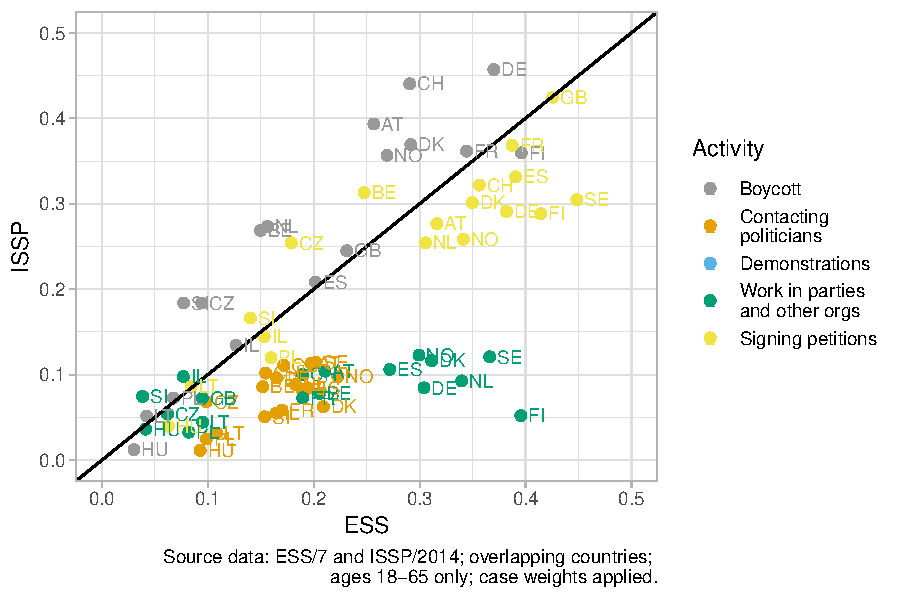
\includegraphics{paper_files/figure-latex/part-rate-dot-plot-1} 

}

\caption{Participation levels in single activities}\label{fig:part-rate-dot-plot}
\end{figure}

\hypertarget{sample-composition-re-weighting-samples}{%
\section{Sample composition: Re-weighting samples}\label{sample-composition-re-weighting-samples}}

To account for possible sample composition differences, weights were calculated to adjust the gender*age*education groups in ISSP to their proportions in the ESS samples. Three age groups were considered - 18-29, 30-49, 50-65 - and three education groups - secondary, post-decondary non-tertiary, and tertiary education. Altogether this makes \(2*3*3=18\) combinations.

Table \ref{tab:sample-re-weighting} shows correlations between sample proportions in the ESS and in the (un-weighted) ISSP, and the same correlations between ESS and ISSP re-weighted to match sample proportions from the ESS. In all cases the correlations with the re-weighted data are weaker, with the largest difference for work in a political party (0.57 compared to 0.34), and smaller declines in the case of the other activities.

\begin{table}[t]

\caption{\label{tab:sample-re-weighting}Correlations between ESS and ISSP participation levels}
\centering
\fontsize{11}{13}\selectfont
\begin{tabular}{lrr}
\toprule
Activity & ESS \& ISSP & ESS \& ISSP re-weighted\\
\midrule
\rowcolor{gray!6}  boycott & 0.929 & 0.906\\
contact & 0.727 & 0.612\\
\rowcolor{gray!6}  demo & 0.915 & 0.901\\
party & 0.565 & 0.341\\
\rowcolor{gray!6}  petition & 0.888 & 0.823\\
\bottomrule
\end{tabular}
\end{table}

\hypertarget{canonical-correlations}{%
\section{Canonical correlations}\label{canonical-correlations}}

In the second attempt a different approach was explored. The question was whether the extent to which political participation is associated with basic socio-demographic variables (age, gender, and education) varies across countries, and whether it is consistent within countries in the two survey projects, ESS and ISSP.

Canonical correlations were calculated for five binary variables corresponding to the five activities on one side, and gender, age (3 categories) and education (3 categories) on the other. Figure \ref{fig:can-cor} shows the correlation coefficients for all countries covered by both ESS and ISSP. The correlation between both series is around 0.2.

\begin{figure}[H]

{\centering 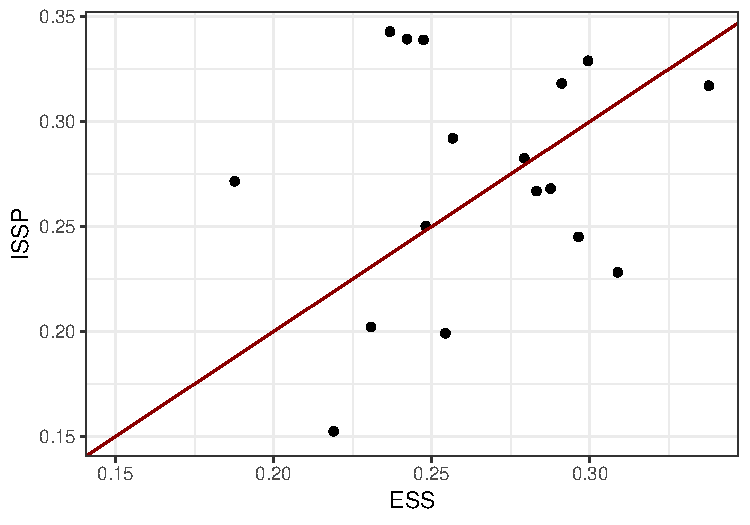
\includegraphics{paper_files/figure-latex/can-cor-1} 

}

\caption{Canonical correlations between participation and sociodemograhics: ESS/7 and ISSP/2014}\label{fig:can-cor}
\end{figure}

\hypertarget{weighted-participation-index}{%
\section{Weighted participation index}\label{weighted-participation-index}}

In the final attempt, political participation was measured as a weighted sum of distinct activities the responded declared having participated in. Four types of weights were considered:

\begin{enumerate}
\def\labelenumi{\arabic{enumi}.}
\tightlist
\item
  The probit of the complement of the participation level: \(probit(1 - p_{i,j})\),\\
\item
  The natural log of the reciprocal of the participation level: \(ln(1 / p_{i,j})\),
\end{enumerate}

where \(p_{i,j}\) is the level of participation in activity \emph{i} in country \emph{j}.

\begin{enumerate}
\def\labelenumi{\arabic{enumi}.}
\setcounter{enumi}{2}
\tightlist
\item
  Ranks according to the estimated effort associated with each activity, in descending order. The rank weights were assigned as follows: work in party or organization (5), participation in demonstrations (4), contacting politicians (3), signing petitions (2), and boycotting (1),\\
\item
  Unit weights (weighted number of activities the respondent participated in),
\end{enumerate}

The fifth political participation indicator to served as a benchmark:
5. A dummy indicating whether the respondent took part in any of the 5 selected activities (coded 1) or if they didn't take part in any (coded 0).

\hypertarget{country-levels-of-overall-political-participation}{%
\subsection{Country levels of overall political participation}\label{country-levels-of-overall-political-participation}}

For each of the five variants of weights the Political Participation Score (PPS) was calculated for each individual. Sample means of PPS for countries that appear in both ESS and in ISSP are shown in Figure \ref{fig:part-level-dot-plot}.

\begin{figure}[H]

{\centering 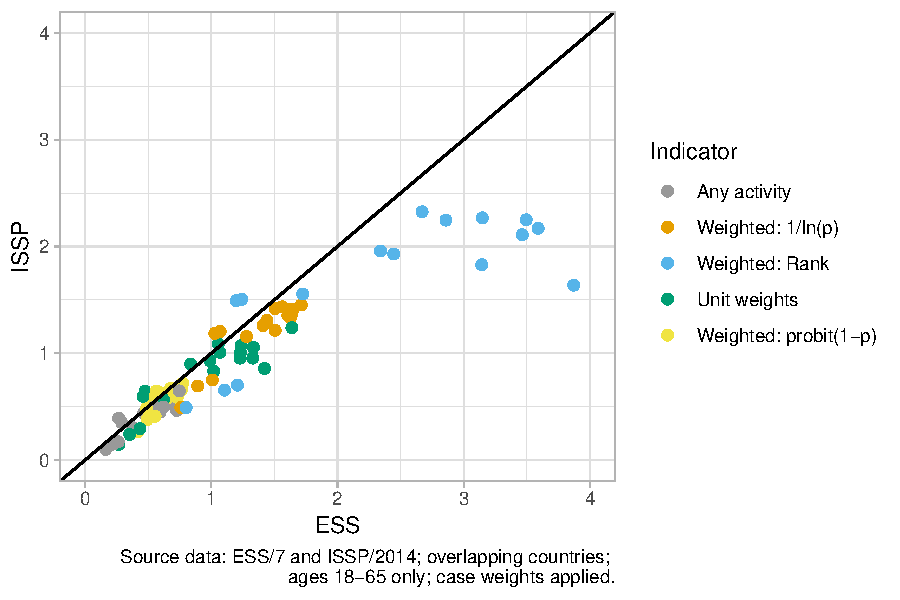
\includegraphics{paper_files/figure-latex/part-level-dot-plot-1} 

}

\caption{Political participation levels by indicator type}\label{fig:part-level-dot-plot}
\end{figure}

\hypertarget{correlations-with-interest-in-politics}{%
\subsection{Correlations with interest in politics}\label{correlations-with-interest-in-politics}}

One way of determining which of the participation measures is best would be to analyze their association with a variable that is known to correlate with political participation. The strongest correlate of political participation is probably interest in politics, although it is not clear what correlation can be reasonably expected other than they should be positive.

Correlations between each of the PPS variants and interest in politics by country range from around 0.21 to 0.43 in the ESS, and from 0.12 and 0.44 in the ISSP. The means are around 0.3 and 0.28, respectively. The differences in correlations across the variants of PPS are very small, and do not clearly favor one or the other variant. On average, in both projects the log of inverse proportion and the unweighted sum fare a little better than the other two variants.

\hypertarget{problems}{%
\section{Problems}\label{problems}}

* the problems will change *

All three measures: the Gini coefficient of political participation constructed as a weighted mean of participation in individual activities, entropy of participation profiles, and the ratio between the proportion of those who participate both in elections and in some other activities divided by the proportion of those who do neither, probably don't measure what they were supposed to measure, but it's hard to know for sure. The problems are conceptual and practical.

It is not clear how to think about political participation as a phenomenon to be quantified, and what aspect of it can or should be quantified: duration, intensity, engagement (and what type?), effectiveness, determination, consequence and consistency, issue-orientedness, or one of the WUNC elements (worthiness, unity, numbers and commitment)? If we saw two instances of participation, would we know which one is larger and which is smaller?
Generally, it is hard to measure that which is not well defined.

The first approach attempts to measure the intensity of political participation by assigning weights to selected five activities, and treating the weighted sum as a metric measure of participation, as required by the Gini coefficient. There are a few ways of thinking about political participation in terms of the sum of activities, for example from the point of view of (1) investment (time and/or money) or the (2) efficiency of the chosen activities. In (1), weights should in principal be different for all individuals, because it takes a different amount of time or money to participate in a demonstration depending on how far from that demonstration one lives, among many other factors. The opportunity cost of participation would be a way of estimating its value. In (2), one would have to be able to estimate the efficiency of different forms of participation.
While it seems reasonable to assume that those activities that require more effort or are otherwise harder to participate in should be weighted more, it is hard to decide how to assign weights without a theoretical or other justification.
Taking a step back, it is not clear why participation in a larger number of activities should count as ``more'' participation than repeated participation in one type of activity. Available survey data typically do not allow to distinguish between one-off and repeated participation in the same activity.

The second measure considers participation profiles (subsets of the analyzed activities individuals engage in) and calculates the amount of information in their distribution across countries. Entropy treats groups as nominal, so changing the group labels on the distribution of the groups would not change the value of entropy, even if substantively the situation changes a lot. For example, if 70\% of people do not demonstrate at all, 20\% sign petitions, and 10\% participate in all five activities, entropy would be the same as if 70\% participated in everything, 20\% did nothing, and 10\% signed petitions. It seems that a measure of inequality of political participation should distinguish between these two situations.

The third measure was a complete experiment. One of the problems of ratios, as reflected in the wide bootstrap confidence intervals, is their sensitivity to small denominators. In countries where the proportion of individuals who do not engage in any activity is very small, the ratio will be large and imprecise.

Generally, measures that rely on means or proportions (like all the three types described earlier) are problematic, because means are sensitive to bias resulting from sampling and other methodological differences across national surveys and survey projects, including differences in question wording. As shown in Table \ref{tab:ind-table}, while the ESS and ISSP ask about the same activities, in almost all cases the wording is slightly different. For example, the ESS mentions ``lawful public demonstrations'' and the ISSP mentions simply ``demonstrations'', and separately asks about ``rallies''. Is a rally a public lawful demonstration? If means (proportions) are not comparable, chances are that any more complex measure that relies on these means (proportions) will also be incomparable.

Three measures of inequality of political participation were experimented with, but were not described in this note. First, the Gini index of the weighted index of participation, turned out to be of little use due to the high proportion of non-participants. The second measure, entropy of participation profiles, treated participation profiles (combinations of participation and non-participation in five activities) as nominal characteristics, without a theoretical reason. The third was the ratio of the proportion of individuals who participated in elections and at least one other activity, divided by the ratio of participants who did neither.


\end{document}
